\chapter{Expériences numériques}
	\minitoc

% Nous allons maintenant nous concentrer sur notre problème de bain (et de baignoire qui fuit). Lors de la recherche de
% comment mettre notre bain en place, nous avons rencontré plusieurs situation.
% Quid:
% \begin{itemize}
% \item Premiers test de bain (boîte sans gravitation, sphère de King...),
% \item Premières conditions semblant cohérente,
% \item Résultat donnés par ces conditions.
% \end{itemize}

Après avoir étudié les propriétés observationnelles des amas globulaires et des galaxies, nous avons mis en évidence un certain nombre
de résultats analytiques sur diverses sphères isothermes. Nous allons maintenant entreprise des simulations numériques visant
à illustrer ces divers résultats et constats.

Les expériences que nous allons mener consistent à étudier la dynamique d'un système auto-gravitant (\textsc{sag}) placé
dans un bain thermique. Les conditions respectent celles du problèmes détaillé dans la section~\ref{Sec::ToyModel}.
% respectant ainsi les conditions du problème détaillé dans la section~\ref{Sec::ToyModel}.
%Nous avons testé plusieurs idées pour mettre en place les conditions décrite dans la section~\ref{Sec::ToyModel}.


Afin de préserver l'intégrité de nos différents systèmes, nous avons imposé aux particules du bain et du \textsc{sag} d'avoir la
même masse.

\section{Description des conditions initiales}

% \subsection{Les différents types de bain}

	Nous avons utilisé principalement deux types de bain:
	\begin{description}

		\item[Le thermostat:] ce type de bain est construit de sorte à se comporter comme un
			thermostat. Il s'agit d'un cube périodique, dans lequel les particules massives sont
			réparties spatialement selon une distribution uniforme. La température est fixée par la
			la distribution gaussienne attribuée aux vitesses. Un thermostat maintient une
			température sans être affecté par le système avec lequel il est en contact.
			% pas supposé échangé autre chose que de l'énergie avec les systèmes en contact,
			Nous faisons donc en sorte que les particules de ce bain puissent influer sur les
			particules du \textsc{sag} sans que celles-ci n'affectent celles du bain en utilisant
			une option de Gadget.
			% , mais ces dernières n'ont aucun effet sur le thermostat.

		\item[Un réservoir thermique:] il s'agit d'un système composé de particules massives réparties
			uniformément dans un cube périodique, et dont la température est aussi fixée par une
			distribution gaussienne des vitesses. Contrairement au thermostat, les particules du
			réservoir ressentent l'interaction gravitationnelle des particules du \textsc{sag}.
		% \item[Un cube homogéne:] il s'agit d'une variante du bain précédant où les particules vont pouvoir subir
			% l'influence du \textsc{sag} placé en leur sein.

		% \item[Une sphère isotherme:] plus précisément, nous allons prendre un modèle de King qui, comme
			% nous l'avons vu dans le chapitre~\ref{King::Chapitre}, est isotherme. Il est
			% donc possible de l'utiliser pour créer un bain thermique, notamment en plaçant le
			% \textsc{sag} au sein de son cœur.

	\end{description}

	Les paramètres du réservoir et du thermostat sont les suivants:
	\begin{itemize}
		\item le nombre de particules $N_b$;
		\item la température $T$;
		\item côté du cube $R_c$.
	\end{itemize}
	Ces paramètres sont indépendants et constituent une partie de l'espace des paramètres de nos
	simulations. La stabilité du réservoir thermique va dépendre des valeurs de ces paramètres, notamment à
	travers le critère de Jeans (voir la section~\ref{Chap::Instabilite::Sec::Jeans}).

	\begin{figure}[hbt]
		\begin{center}
			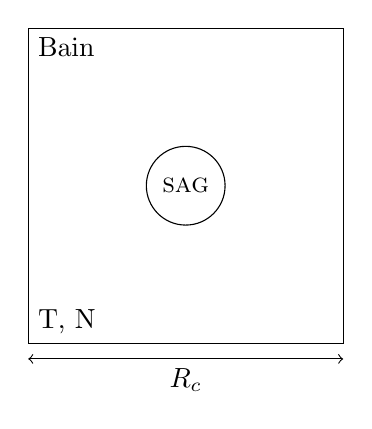
\begin{tikzpicture}
				\draw (0, 0) circle (0.5);
				\node at (0, 0) {\textsc{sag}};

				\draw (-2, 2) rectangle (2, -2);
				\node at (-2, 2) [below right] {Bain};
				\node at (-2, -2) [above right] {T, N};
				\draw[<->] (-2, -2.2) -- (2, -2.2);
				\node at (0, -2.2) [below] {$R_c$};
			\end{tikzpicture}
			\caption{Condition des simulations.\label{Fig::CI::Repr}}
		\end{center}
	\end{figure}

	L'effet d'un thermostat sur le \textsc{sag} ne peut a priori se faire qu'aux travers des collisions, les
	particules du thermostat ne pouvant être capturé par le \textsc{sag}. L'effet correspondant ne peut
	alors apparaître que sur des temps grand devant le temps dynamique du \textsc{sag} (voir-- mettre le
	lien vers la discussion correspondante, une fois écrite). Un réservoir thermique sera à priori plus
	efficace, les interactions gravitationnelles pouvant amener une partie des particules du réservoir à
	être capturé par le \textsc{sag}, ou réciproquement. Des effets peuvent donc apparaître plus rapidement.

	Nous avons utilisé deux types de \textsc{sag}:
	\begin{itemize}
		\item un modèle de King, de paramètre $W_0$, $\sigma$, $r_c$ et $N_K$;
		\item une sphère de Hénon, de paramètre $R$, $M$, $\gamma$ et $N_H$.
	\end{itemize}

	La figure~\ref{Fig::CI::Repr} représente la répartition initiale du bain et du \textsc{sag}. À ce moment, des particules du bain se trouvent déjà dans le \textsc{sag}.

% \subsection{Réalisation du système}

\section{Étude préliminaire}

% \subsection{King dans bain sans interaction}

	Une première série de simulation du système à consisté à placer un modèle de King, de paramètre $W_0 = 5.2$, $\sigma_c = 2.9\
	\mathrm{km}.\mathrm{s}^{-1}$ et $r_c = 3.5\ \mathrm{pc}$, dans un thermostat. Les paramètres de chaque simulations étaient la
	température du bain, la taille de la boîte et le nombre de particule utilisées dans chacun des deux systèmes. La taille de la boîte
	nous permet de jouer sur la densité du bain. La température était calculée pour être un multiple $k$ de la température moyenne de la
	sphère de King initiale. Nous avons fait varier $k$ dans l'intervalle $10^{-3}$ à $10^5$. Chaque configuration initiale a évolué
	sur des périodes de temps allant de $10T_d$ à $120T_d$, où $T_d$ est le temps dynamique de la sphère de King initiale (voir le
	chapitre~\ref{Chap::TempsCarac})
	% de $10^{-3}T_\mathrm{Bord}$ à $10^5 T_\mathrm{Centre}$.
	La densité du \textsc{sag} n'a jamais montré de véritable évolution, ni les autres paramètres.

	PLACER QUELQUES GRAPHES.

	% Ceci est dû au fait que le bain ne peut changer la dispersion de
	% vitesse des particules du King que lors de collision à plusieurs corps. Or ces collisions sont assez
	% longue à agir.

	% Une première représentation du système consiste à placer un modèle de King dans un thermostat. Les
	% paramètres du King ont été fixé à $W_0 = 5.19773$, $\sigma_c = 2.9\ \mathrm{km}.\mathrm{s}^{-1}$ et $r_c
	% = 3.5\ \mathrm{pc}$. Les paramètres de chaque simulations
	% étaient la température du bain, la taille de la boîte et le nombre de particule utilisé dans chacun des
	% deux systèmes. La taille de la boîte nous permet de jouer sur la densité du bain. La température était
	% calculer pour être un multiple soit de la température du cœur de la sphère de King soit un multiple de
	% sa température moyenne. Nous avons parcouru des température allant de $10^{-3}T_\mathrm{Bord}$ à $10^5
	% T_\mathrm{Centre}$. La densité n'a jamais montré de véritable évolution, ni les autres paramètres.
	% Ceci est dû au fait que le bain ne peut changer la dispersion de vitesse des particules du King que lors
	% de collision à plusieurs corps. Or ces collisions sont assez longue à agir.

	% La première idée que nous avons testé tentait de simuler un véritable bain thermique. Nous placions un
	% modèle de King dans une boîte périodique rempli de particule répartie de façon homogène et placé à une
	% certaine température.
	% Par \og simuler un véritable bain thermique\fg nous entendons que les particules du bain ne peuvent pas
	% se faire capturer par le Kingi, mais elles peuvent modifier la vitesse des particules de ce dernier.
	% % C'est-à-dire que le bain pouvait influer sur la vitesse des
	% Au final, ces simulations n'ont jamais rien donnée car...

% \subsection{King dans un King}

	% Une seconde représentation consiste à placer un modèle de King dans une sphère isotherme qui fera office de
	% bain. Nous faisons en sorte que le King soit contenu dans le cœur du bain, dont les paramètres ont été
	% choisi de sorte à ce que le cœur soit complètement isotherme. Un problème est très vite arrivé: pour que
	% le bain ait un cœur suffisamment grand pour contenir le \textsc{sag}, il fallait qu'il ait une taille
	% tellement grande que le nombre de particule nécessaire pour avoir quelque chose de correct était de
	% l'ordre de $10^{10}$ particules.

	% Nos pérégrination nous ont ensuite mené à tenter de simuler le bain non plus par un cube, mais par une
	% autre sphère isotherme, en l'occurrence un autre King. L'idée était de générer un King dont le cœur
	% était suffisamment grand pour y faire tenir un autre King, et le mettre à la bonne température. Le gros
	% souci auquel nous avons eu à faire, c'est que le King devant servir de bain se trouvait être très dilué.

% \subsection{Hénon dans un King}

	% Une troisième approche nous est venu en se disant que, si le king n'évoluait pas, c'est parce qu'il
	% était trop stable, ou que son temps dynamique était trop grand. Nous somme donc passé sur une autre
	% catégorie de \textsc{sag}: ceux formés suite à l'effondrement d'une sphère de Hénon. Il s'agit donc ici
	% de remplacer nos modèle de King par une sphère de Hénon qui, après effondrement, va devenir un cœur-halo
	% avec une pente de $-4$. Les conditions que nous imposons pour ces simulations font que le bain doit
	% avoir une température égale ou inférieur au \textsc{sag}. Or, le \textsc{ch4} était trop froid pour que
	% nous puissions mettre le King à la bonne température.

	% Après les résultats décevant des CI précédentes, nous nous sommes dit que le King était peut-être trop
	% stable, et du coups l'instabilité se produit après des temps trop long. Nous avons donc choisi de donner
	% sa chance à la sphère de Hénon en espérant que le premier effondrement (dû à l'instabilité de Jeans)
	% permette l'apparition rapide de l'instabilité souhaité. Pour diverses raisons dû à la température, nous
	% avons abandonné cette idée.

% \subsection{Hénon dans un cube}

	% La dernière approche à laquelle nous ayons pensé est de rester avec un Hénon, mais cette fois placé dans
	% un cube homogène. Le bain interagissant pleinement avec le \textsc{sag}, ce dernier va pouvoir accréter
	% ou perdre de la masse en interagissant avec le bain, accélérant par là son évolution. Nous avons pu
	% observer plusieurs phénomènes intéressant que nous allons détailler dans la prochaine section.

	% Une autre approche a été développé, consistant à remplacer le thermostat par un réservoir thermique.
	% Nous allons aussi remplacer le modèle de King par une sphère de Hénon.
	% C'est sur cet ensemble de simulations que nous allons nous concentrer dans la suite.

	Face à ce constat, nous avons augmenté la sensibilité de nos simulations en remplaçant le thermostat par un réservoir thermique et la
	sphère de King par une sphère de Hénon.

	% Nous avons finalement décidé de revenir à l'idée initiale, mais avec deux changements majeurs: cette
	% fois le bain va subir l'influence de la gravitation, et nous avons remplacé la \textsc{sik} par une
	% sphère de Hénon. Pourquoi ce changement pour le bain? Parce que nous avons réalisé que le meilleurs
	% moyen de jouer sur la température de notre \textsc{si} est de la laisser acquérir des particules du bain
	% afin de changer la profondeur de son puits de potentiel et donc sa température.
	% Cette configuration nous a permis de mettre en évidence plusieurs évolutions intéressante, mais toujours
	% pas l'instabilité que nous cherchions.

	% Nous allons détailler dans les sections suivantes les conditions de ce set-up et les premiers résultats
	% obtenu ainsi.

\section{Seconde étude}

% \subsection{Comment elles sont mise en place}

	% Pour commencer, nous nous plaçons dans le même système d'unité que celui du
	% chapitre~\ref{Chap::VlasovGadget}. Une première étape est de chercher quels contrainte nous voulons
	% imposer aux différents objet de la simulation. La première étape est bien entendu de s'assurer que les
	% conditions périodiques n'influe pas trop sur l'évolution. Ensuite, nous aimerions imposer aussi la taille de
	% la boîte de sorte que le bain soit stable. Il se trouve que ces deux conditions sont parfois
	% incompatible, la boîte devant être petite pour assurer la stabilité mais pas assez grande pour éviter
	% les soucis inhérents aux conditions périodiques. D'autant que nous devons conserver la température du
	% bain inférieur à celle de la sphère de Hénon une fois effondré.

	% Nous avons fini par choisir de faire sauter la conditions sur la taille de la boîte, ce qui nous fait
	% gagner un paramètre en plus sur lequel jouer plus facilement. Nous avons ensuite lancé un grand nombre
	% de simulations pour parcours une partie de l'espace des paramètres et voir ce qu'il se passe.

	Une seconde série de simulation est construite en utilisant une sphère Hénon de rayon $R=2$, de masse $M=1$ et de viriel $\gamma=-0,5$ placée
	dans un réservoir thermique. Nous utiliserons ici le même système d'unité que dans le chapitre~\ref{Chap::VlasovGadget}, ainsi le temps
	dynamique du \textsc{sag} est $T_d^H = 2\pi$ dans ces unités. Comme pour l'étude précédente, nous allons utiliser comme paramètres des
	simulations les paramètres du réservoir: le nombre de particules $N_b$, la taille du cube $R_c$ et sa température $\sigma_c$. Globalement
	l'évolution dynamique de ce système montre toujours deux phases successives. Dans un premier temps, la sphère de Hénon s'effondre et forme,
	comme attendu pour $\gamma=-0,5$, une structure cœur-halo de $\alpha\simeq-4$ (\textsc{ch4}) à l'équilibre ($\gamma=-1$). La durée de cette
	phase initiale est de l'ordre de quelques temps dynamiques de la sphère de Hénon initiale. Cette phase d'effondrement n'est globalement pas
	affecté par les paramètres du réservoir. L'intersection des deux systèmes (bain et \textsc{sag}) n'étant pas vide, le nombre de particules du
	bain contenu dans le \textsc{sag} va quelque peu varier, changeant sensiblement quelques paramètres après l'effondrement. La
	figure~\ref{Fig::Simu::EvoParamPostCollapse} illustre l'évolution, après effondrement, des différents rayons, axes d'inertie, viriel,
	température et anisotropie en fonction des paramètres du réservoir thermique. Cette phase d'effondrement est la traduction de l'instabilité de
	Jeans.
	% par le nombre de particules du bain (l'intersection des deux système n'étant pas vide). Globalement, le premier effondrement du Hénon, sous
	% l'influence de l'instabilité de Jeans, se déroule sans aucun effet dû à la présence du Bain.

	L'évolution dynamique post-effondrement de cette structure de type \textsc{ch4} est alors influencé par le bain. Cette influence est modulée
	par les paramètres du réservoir thermique. La table~\ref{Tab::SimuZoomRes} résume l'évolution d'une partie des simulations qui ont été faîtes.
	Les notations utilisées sont les suivantes:
	\begin{description}
		\item[les notations] sont les mêmes que dans le chapitre~\ref{Chap::Simu::Analysis};
		\item[$diamondsuit$] indique une triaxialisation du système;
		\item[\accretionpeu{}] indique un "effondrement" de l'objet et correspond à la variation suivante des différents rayons;
			$\Delta \ra<0\%$, $\Delta \rb<0\%$, $\Delta \rc<100\%$;
		\item[\accretionmoyen{}]  indique une accrétion "moyenne" du bain par le \textsc{sag} et correspond à la variation suivante des
			différents rayons: $\Delta \ra<0\%$, $0\%<\Delta \rb<100\%$, $\Delta \rc<100\%$;
		\item[\accretionlot{}] indique une forte accrétion du bain par le \textsc{sag} et correspond à la variation suivante des différents
			rayons: $\Delta \ra>200\%$, $\Delta \rb>200\%$, $\Delta \rc>200\%$;
		\item[$\emptyset$] indique que le ou les paramètres n'ont pas évoluer de manière significative.
	\end{description}
	% $a_1 = \lambda_1 / \lambda_2$, $a_2 = \lambda_3 / \lambda_2$; $\lambda_1>\lambda_2>\lambda_3$. Accrétion:
	% \begin{description}
		% % \item[\contraction{}] -> $\Delta r_{10\%}<0$, $\Delta r_{50\%}<0$, $\Delta r_{90\%}<0$,
		% \item[\accretionpeu{}] indique un "effondrement" de l'objet et correspond à la variation suivante des différents rayons: $\Delta \ra<0\%$, $\Delta \rb<0\%$, $\Delta \rc<0\%$,
		% \item[\accretionmoyen{}]  indique un "effondrement" de l'objet et correspond à la variation suivante des différents rayons: $0\%<\Delta \ra<200\%$, $0\%<\Delta \rb<200\%$, $0\%<\Delta \rc<200\%$,
		% \item[\accretionlot{}] -> $\Delta \ra>200\%$, $\Delta \rb>200\%$, $\Delta \rc>200\%$.
	% \end{description}

	% Ensuite, les résultats sont assez variables. Toutes les simulations montrent un réchauffement du
	% Hénon, mais relativement peu indiquent une évolution des autres paramètres, tel l'anisotropie où les axes d'inertie. La
	% table~\ref{Tab::SimuZoomRes} montre un résumé de certaines de ces simulations.

	\begin{figure}[htbp]
		\centering \rotatebox{90}{
			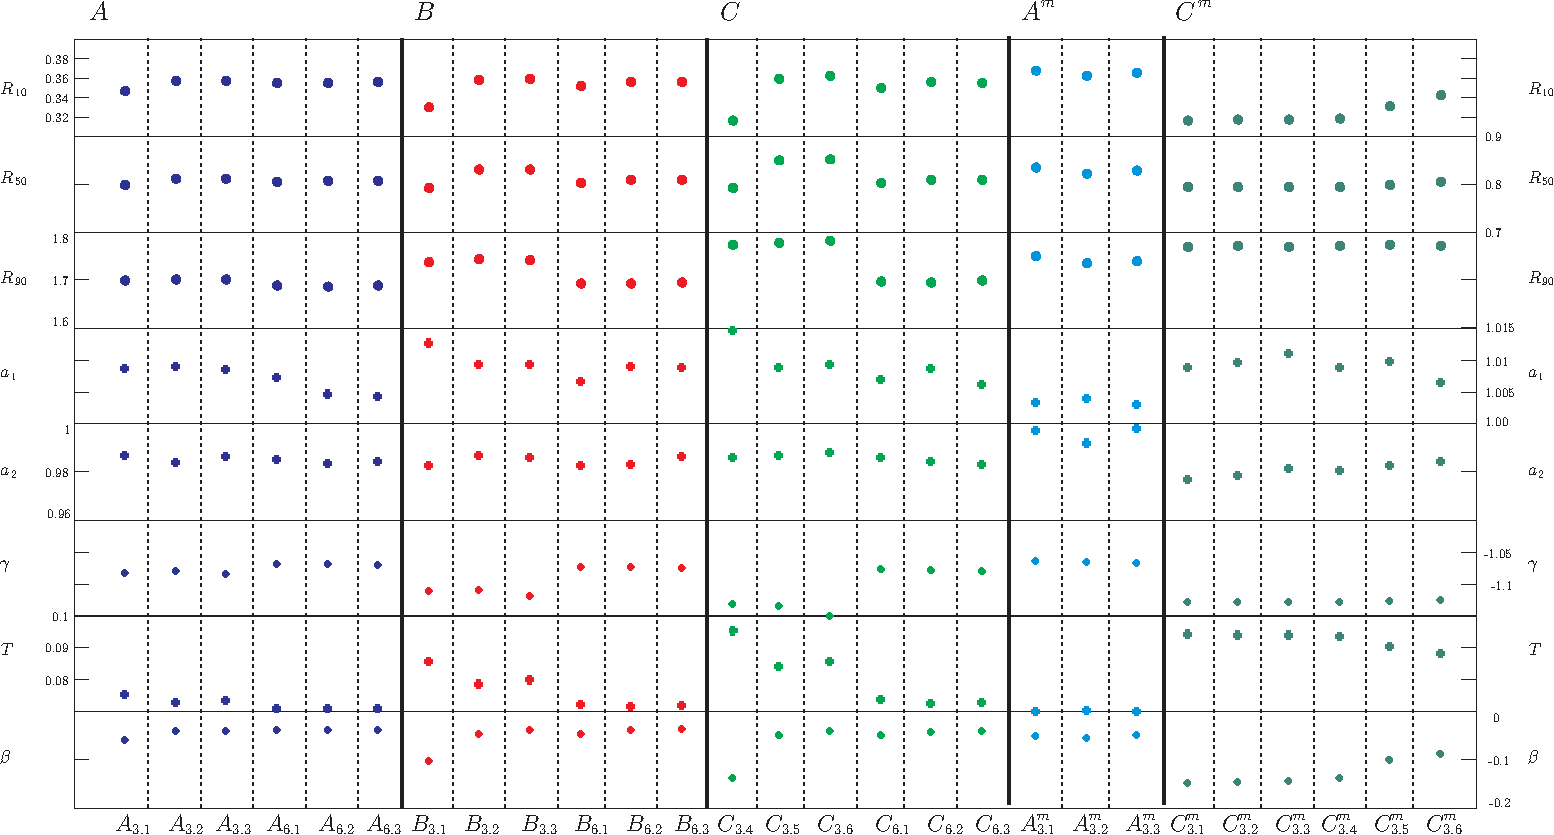
\includegraphics[scale=0.8]{graphe/post-collapse.pdf}
		}
		\caption{Évolution des différentes observable après l'effondrement en fonction des paramètres du bain thermique.\label{Fig::Simu::EvoParamPostCollapse}}
	\end{figure}

	\begin{table}[htbp]
		% \begin{tabular}{|m{1.5cm}|m{1cm}|m{2cm}|m{2cm}|m{2.5cm}|m{2.0cm}|m{2cm}|}
	% Vérifier la pente du halo et ajouter celle du centre
	\centering
		\begin{tabular}{|c|c|c|c|c|c|c|c|c|c|}
			\hline $N$ & $R_c$ & $\sigma_c$ & $R_{10}$, $R_{50}$, $R_{90}$ & $a_1$, $a_2$ & $\beta$ & $\rho$ & $T$ & $\gamma$ & nom \tabularnewline
			\hline
			\hline \multirow{6}{*}{$1\ 10^5$} & \multirow{3}{*}{$33.3$}
					% & $10^{-3}$ & Accrétion & Triaxialisation du \textsc{sag} & tend vers $-0,5$ & Évolution de la pente du halo \tabularnewline \cline{3-7}
					% & $10^{-3}$ & Accrétion & \begin{tikzpicture}\node[draw,ellipse] at (0,0) {}; \end{tikzpicture}Triaxialisation du \textsc{sag} & tend vers $-0,5$ & Évolution de la pente du halo \tabularnewline \cline{3-7}
					& $10^{-3}$ & \accretionmoyen{} & $\diamondsuit$ & ${}_{0.15}\nearrow^{0.43}$ & $\alpha\searrow$ & $\nearrow$ & $\searrow$ & $A_{3,1}$ \tabularnewline \cline{3-10}
					& & $10^{-1}$ & \accretionpeu{} & $\emptyset$ & ${}^{0.02}\searrow_{-0.1}$ & $\emptyset$ & $\nearrow$ & $\emptyset$ & $A_{3,2}$  \tabularnewline \cline{3-10}
					& & $2\ 10^{-1}$ & \accretionpeu{} & $\emptyset$ & ${}^{0.02}\searrow_{-0.11}$ & $\emptyset$ & $\nearrow$ & $\emptyset$ & $A_{3,3}$  \tabularnewline \cline{2-10}
				& \multirow{3}{*}{$66.6$}
					& $10^{-3}$ & \accretionpeu{} & $\emptyset$ & ${}^{0.08}\searrow_{0.03}$ & $\emptyset$ & $\nearrow$ & $\searrow$ & $A_{6,1}$  \tabularnewline \cline{3-10}
					& & $10^{-1}$ & \accretionpeu{} & $\emptyset$ & ${}^{0.06}\searrow_{-0.11}$ & $\emptyset$ & $\nearrow$ & $\emptyset$ & $A_{6,2}$  \tabularnewline \cline{3-10}
					& & $2\ 10^{-1}$ & \accretionpeu{} & $\emptyset$ & ${}^{0.06}\searrow_{-0.12}$ & $\emptyset$ & $\nearrow$ & $\emptyset$ & $A_{6,3}$  \tabularnewline \cline{2-10}
			\hline
			\hline $2\ 10^5$ & $66.6$ & $10^{-3}$ & \accretionpeu{} & $\emptyset$ & ${}_{0.1}\nearrow^{0.17}$ & $\alpha\searrow$ & $\nearrow$ & $\emptyset$ & $A_{6,1}^m$  \\
			\hline
			\hline $4\ 10^5$ & $66.6$ & $10^{-3}$ & \accretionpeu{} & $\emptyset$ & ${}_{0.1}\nearrow^{0.23}$ & $\alpha\searrow$ & $\nearrow$ & $\emptyset$ & $A_{6,2}^m$  \\
			\hline
			\hline $1\ 10^6$ & $66.6$ & $10^{-3}$ & \accretionpeu{} & $\emptyset$ & ${}_{0.12}\nearrow^{0.27}$ & $\alpha\searrow$ & $\nearrow$ & $\emptyset$ & $A_{6,3}^m$  \\
			\hline
			\hline \multirow{6}{*}{$3.25\ 10^5$} & \multirow{3}{*}{$33.3$}
					& $10^{-3}$ & \accretionlot{} & $\spadesuit$ & ${}^{0.36}\searrow_{0.33}$ & $\alpha\searrow$ & $\nearrow$ & $\searrow$ & $B_{3,1}$  \tabularnewline \cline{3-10}
					& & $10^{-1}$ & \accretionpeu{} & $\emptyset$ & ${}^{0.05}\searrow_{0.0}$ & $\emptyset$ & $\nearrow$ & $\searrow$ & $B_{3,2}$  \tabularnewline \cline{3-10}
					& & $2\ 10^{-1}$ & \accretionpeu{} & $\emptyset$ & ${}^{0.03}\searrow_{-0.05}$ & $\emptyset$ & $\nearrow$ & $\emptyset$ & $B_{3,3}$  \tabularnewline \cline{2-10}
				& \multirow{3}{*}{$66.6$}
					& $10^{-3}$ & \accretionpeu{} & $\emptyset$ & ${}_{0.11}\nearrow^{0.42}$ & $\alpha\searrow$ & $\nearrow$ & $\searrow$ & $B_{6,1}$  \tabularnewline \cline{3-10}
					& & $10^{-1}$ & \accretionpeu{} & $\emptyset$ & ${}^{0.06}\searrow_{-0.1}$ & $\emptyset$ & $\nearrow$ & $\emptyset$ & $B_{6,2}$  \tabularnewline \cline{3-10}
					& & $2\ 10^{-1}$ & \accretionpeu{} & $\emptyset$ & ${}^{0.06}\searrow_{-0.1}$ & $\emptyset$ & $\nearrow$ & $\emptyset$ & $B_{6,3}$  \tabularnewline \cline{2-10}
			\hline
			\hline \multirow{6}{*}{$5.5\ 10^5$} & \multirow{3}{*}{$33.3$}
					& $10^{-3}$ & \accretionlot{} & $\spadesuit$ & ${}_{0.5}\nearrow^{0.37}$ & $\alpha\searrow$ & $\nearrow$ & $\searrow$ & $C_{3,4}$  \tabularnewline \cline{3-10}
					& & $10^{-1}$ & \accretionlot{} & $\emptyset$ & ${}^{0.07}\searrow_{0.03}$ & $\emptyset$ & $\nearrow$ & $\searrow$ & $C_{3,5}$  \tabularnewline \cline{3-10}
					& & $2\ 10^{-1}$ & \accretionpeu{} & $\emptyset$ & ${}^{0.04}\searrow_{-0.01}$ & $\emptyset$ & $\nearrow$ & $\searrow$ & $C_{3,6}$  \tabularnewline \cline{2-10}
				& \multirow{3}{*}{$66.6$}
					& $10^{-3}$ & \accretionmoyen{} & $\spadesuit$ & ${}_{0.15}\nearrow^{0.67}$ & $\alpha\searrow$ & $\nearrow$ & $\searrow$ & $C_{6,1}$  \tabularnewline \cline{3-10}
					& & $10^{-1}$ & \accretionpeu{} & $\emptyset$ & ${}^{0.06}\searrow_{-0.07}$ & $\emptyset$ & $\nearrow$ & $\emptyset$ & $C_{6,2}$  \tabularnewline \cline{3-10}
					& & $2\ 10^{-1}$ & \accretionpeu{} & $\emptyset$ & ${}^{0.05}\searrow_{-0.1}$ & $\emptyset$ & $\nearrow$ & $\emptyset$ & $C_{6,3}$  \tabularnewline \cline{2-10}
			\hline
			\hline \multirow{6}{*}{$1856250$} & \multirow{6}{*}{$50$}
					& $1,25\ 10^{-4}$ & \accretionlot{} & $\spadesuit$ & ${}^{0.5}\searrow_{0.13}$ & $\alpha\searrow$ & $\nearrow$ & $\searrow$ & $C_{3,1}^m$  \tabularnewline \cline{3-10}
					& & $2,5\ 10^{-4}$ & \accretionlot{} & $\spadesuit$ & ${}^{0.5}\searrow_{0.28}$ & $\alpha\searrow$ & $\nearrow$ & $\searrow$ & $C_{3,2}^m$  \tabularnewline \cline{3-10}
					& & $5\ 10^{-4}$ & \accretionlot{} & $\spadesuit$ & ${}^{0.5}\searrow_{0.22}$ & $\alpha\searrow$ & $\nearrow$ & $\searrow$ & $C_{3,3}^m$  \tabularnewline \cline{3-10}
					& & $10^{-3}$ & \accretionlot{} & $\spadesuit$ & ${}^{0.5}\searrow_{0.24}$ & $\alpha\searrow$ & $\nearrow$ & $\searrow$ & $C_{3,4}^m$  \tabularnewline \cline{3-10}
					& & $10^{-1}$ & \accretionlot{} & $\emptyset$ & ${\scriptstyle 0.36}\to{\scriptstyle 0.36}$ & $\alpha\searrow$ & $\nearrow$ & $\searrow$ & $C_{3,5}^m$  \tabularnewline \cline{3-10}
					& & $2\ 10^{-1}$ & \accretionlot{} & $\emptyset$ & ${}_{0.3}\nearrow^{0.36}$ & $\emptyset$ & $\nearrow$ & $\searrow$ & $C_{3,6}^m$  \tabularnewline \cline{2-10}
			\hline
		\end{tabular}
	\caption{Résultats des simulations combinant un Hénon et un réservoir thermique.\label{Tab::SimuZoomRes}}
\end{table}



	Certaines simulations montrent des effets dus aux cubes périodiques trop petit. Nous observerons par exemple la simulation $N_b = 10^5$, $R_c
	= 33,3$ et $\sigma_c = 10^{-3}$ qui montre une triaxialisation du \textsc{sag}. La figure~\ref{Fig::Projection::TriAxial} montre l'état de ce
	système à la fin de la simulation qui a duré $15T_d^H$. L'objet montre une forme quasiment cubique et des \og bras\fg partent vers les bords du
	cube, marque des conditions périodiques. Bien qu'il n'y ait que peu de particules dans ces \og bras\fg, nous souhaitons tout de mêmes éviter
	les conditions qui éviteraient de voir apparaître de tel propriété.

	\begin{figure}[hbtp]
		\begin{minipage}{0.48\linewidth}
			\centering 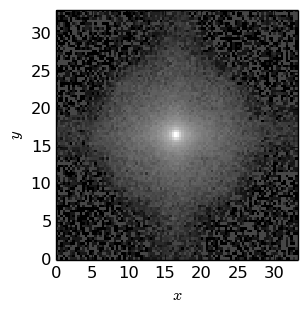
\includegraphics{{graphe/N-100000.0_Rc-33.3333333333_sc-0.001_Soft-0.001_100_xy}.png}
		\end{minipage}\hfill
		\begin{minipage}{0.48\linewidth}
			\centering 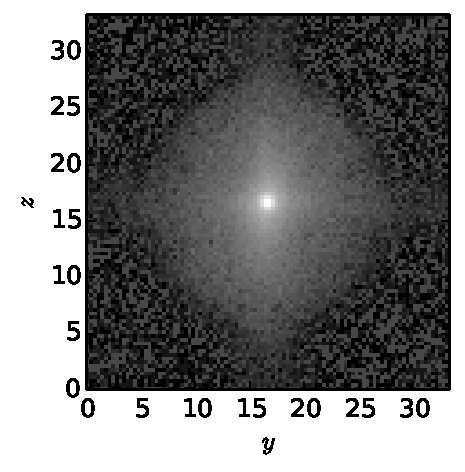
\includegraphics{{graphe/N-100000.0_Rc-33.3333333333_sc-0.001_Soft-0.001_100_yz}.png}
		\end{minipage}
		\centering 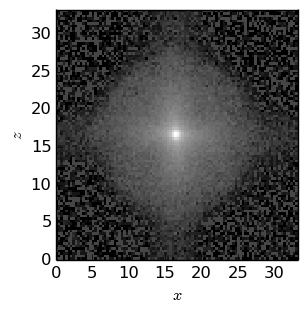
\includegraphics{{graphe/N-100000.0_Rc-33.3333333333_sc-0.001_Soft-0.001_100_xz}.png}
		\caption{Projection de la simulation $N = 10^5$, $R_c = 33,3$ et $\sigma_c = 10^{-3}$\label{Fig::Projection::TriAxial}}
		Ajouter les colorbar de chaque graphes.
	\end{figure}

	D'autres ont montré des effets beaucoup plus intéressants. Prenons la simulation $N_b = 1856250$, $R_c = 50$, $\sigma_c = 10^{-3}$, dont
	l'évolution de certains paramètres est représenté sur la figure~\ref{Fig::Simu::p4s125}. L'évolution des rayons à $10\%$, $50\%$ et $90\%$ de
	masse nous indique une forte accrétion du bain par le \textsc{sag}. Les axes d'inertie semblent indiquer qu'une instabilité d'orbite radiale
	se produise vers $t=30$ (soit $4T_d^H$).

	% \subsection{Qu'avons-nous vu}

	% Et bien, comme prévu, lors de boîte trop petite nous avons les effets des conditions périodiques. Par
	% contre, dans les cas où la taille de la boîte n'était pas suffisante pour assurer la stabilité du bain,
	% nous avons commencer à observer des effets intéressants lié à l'accrétion du bain par l'objet. Dans
	% d'autre cas, où nous n'avions pas assez de particules pour moyenner les effets de relaxations à
	% $N$-corps, nous avons pu voir une évolution intéressante de l'objet. Dans la plupart des cas, il ne
	% c'est rien passez, ou alors uniquement des effets dû à la boîte périodique \& co.

	% \todo[inline]{
		% Mettre les simulations suivantes:
		% \begin{itemize}
			% \item $N = 550 000$, $R_c = 66.6666$, $\sigma_c = 0.001$;
			% \item $N = 550 000$, $R_c = 33.3333$, $\sigma_c = 0.001$ et variante;
			% \item $N = 325 000$, $33.3333$, $\sigma_c = 0.001$.
		% \end{itemize}
	% }

\section{Focalisation sur les simulations intéressantes}

	\subsection{Instabilité d'orbite radiale}

		\begin{figure}[htbp]
			\begin{minipage}{0.45\linewidth}
				\centering \includegraphics{{N-550000.0p1.5p1.5p1.5_Rc-33.3333333333p1.5_sc-0.000125_axial}.pdf}
				\caption{Évolution des rapports d'axes}
			\end{minipage}\hfill
			\begin{minipage}{0.45\linewidth}
				\centering \includegraphics{{N-550000.0p1.5p1.5p1.5_Rc-33.3333333333p1.5_sc-0.000125_rayon}.pdf}
				\caption{Évolution des rayons à $10\%$, $50\%$ et $90\%$ de masse.}
			\end{minipage}
			\caption{Simulation de paramètre $N = 1856250$, $R_c = 49.999999999$, $\sigma_c = 0.000125$.\label{Fig::Simu::p4s125}}
		\end{figure}
		\begin{figure}[htbp]
			\begin{minipage}{0.45\linewidth}
				\centering \includegraphics{{N-550000.0p1.5p1.5p1.5_Rc-33.3333333333p1.5_sc-0.000125_axial}.pdf}
				\caption{Évolution des rapports d'axes pour la simulation de paramètre $N = 1856250$, $R_c = 49.999999999$, $\sigma_c = 0.000125$.}
			\end{minipage}\hfill
			\begin{minipage}{0.45\linewidth}
				\centering \includegraphics{{N-550000.0p1.5p1.5p1.5_Rc-33.3333333333p1.5_sc-0.0005_axial}.pdf}
				\caption{Évolution des rapports d'axes pour la simulation de paramètre $N = 1856250$, $R_c = 49.999999999$, $\sigma_c = 0.0005$.}
			\end{minipage}
				\centering \includegraphics{{N-550000.0p1.5p1.5p1.5_Rc-33.3333333333p1.5_sc-0.001_axial}.pdf}
				\caption{Évolution des rapports d'axes pour la simulation de paramètre $N = 1856250$, $R_c = 49.999999999$, $\sigma_c = 0.001$.}
		\end{figure}
		\begin{figure}[htbp]
			\begin{minipage}{0.45\linewidth}
				\centering \includegraphics{{N-550000.0p1.5p1.5p1.5_Rc-33.3333333333p1.5_sc-0.000125_rayon}.pdf}
				\caption{Évolution des rayons à $10\%$, $50\%$ et $90\%$ de masse pour la simulation de paramètre $N = 1856250$, $R_c = 49.999999999$, $\sigma_c = 0.000125$.}
			\end{minipage}\hfill
			\begin{minipage}{0.45\linewidth}
				\centering \includegraphics{{N-550000.0p1.5p1.5p1.5_Rc-33.3333333333p1.5_sc-0.0005_rayon}.pdf}
				\caption{Évolution des rayons à $10\%$, $50\%$ et $90\%$ de masse pour la simulation de paramètre $N = 1856250$, $R_c = 49.999999999$, $\sigma_c = 0.0005$.}
			\end{minipage}
				\centering \includegraphics{{N-550000.0p1.5p1.5p1.5_Rc-33.3333333333p1.5_sc-0.001_rayon}.pdf}
				\caption{Évolution des rayons à $10\%$, $50\%$ et $90\%$ de masse pour la simulation de paramètre $N = 1856250$, $R_c = 49.999999999$, $\sigma_c = 0.001$.}
		\end{figure}

	\subsection{Évolution de la pente avec l'âge (effet de relaxation)}
		
		\begin{figure}[htbp]
			\begin{minipage}{0.45\linewidth}
				\centering \includegraphics{{N-100000.0_Rc-66.6666666666_sc-0.001_Soft-0.001_axial}.pdf}
				\caption{Évolution des rapports d'axes.}
			\end{minipage}\hfill
			\begin{minipage}{0.45\linewidth}
				\centering \includegraphics{{N-100000.0_Rc-66.6666666666_sc-0.001_Soft-0.001_aniso}.pdf}
				\caption{Évolution de l'anisotropie moyenne du système.}
			\end{minipage}

			\begin{minipage}{0.45\linewidth}
				\centering \includegraphics{{N-100000.0_Rc-66.6666666666_sc-0.001_Soft-0.001_rayon}.pdf}
				\caption{Évolution des rayons à $10\%$, $50\%$ et $90\%$ de masse.}
			\end{minipage}\hfill
			\begin{minipage}{0.45\linewidth}
				\centering \includegraphics{{N-100000.0_Rc-66.6666666666_sc-0.001_Soft-0.001_densite}.pdf}
				\caption{Évolution de la densité à différent temps.}
			\end{minipage}
			\caption{Simulation de paramètre $N=100000$, $R_c=66.6$, $\sigma_c=0.001$.}
		\end{figure}
				\begin{table}[htbp]
			\rotatebox{90}{
				\begin{tabular}{|c|c|c|p{2cm}|p{2cm}|p{2cm}|p{2.0cm}|c|c|c|}
				\hline $N$ & $R_c$ & $\sigma_c$ & $r_{10\%}$, $r_{50\%}$, $r_{90\%}$ & Axial ratio & $\gamma$ & $\beta$ & $T$ & $E$ & $\rho$ \tabularnewline
				\hline \multirow{6}{*}{$1\ 10^5$} & \multirow{3}{*}{$33,3$}
						% & $1,25\ 10^{-4}$ & Rien & rien & $-1$ & rien & rien & rien & Rien \tabularnewline \cline{3-10}
						% & & $2,5\ 10^{-4}$ & Rien & rien & $-1$ & rien & rien & rien & Rien \tabularnewline \cline{3-10}
						% & & $5\ 10^{-4}$ & Rien & rien & $-1$ & rien & rien & rien & Rien \tabularnewline \cline{3-10}
						& $10^{-3}$ & Un poil d'accrétion & Triaxialisation du \textsc{sag} & $-1,4$ & tend vers $-0,5$ & rien & rien & Diminution de la pente du halo \tabularnewline \cline{3-10}
						& & $10^{-1}$ & Rien & rien & $-1$ & rien & rien & rien & Rien \tabularnewline \cline{3-10}
						& & $2\ 10^{-1}$ & Rien & rien & $-1$ & rien & rien & rien & Rien \tabularnewline \cline{2-10}
					& \multirow{3}{*}{$66,6$}
						% & $1,25\ 10^{-4}$ & Rien & rien & $-1$ & rien & rien & rien & Rien \tabularnewline \cline{3-10}
						% & & $2,5\ 10^{-4}$ & Rien & rien & $-1$ & rien & rien & rien & Rien \tabularnewline \cline{3-10}
						% & & $5\ 10^{-4}$ & Rien & rien & $-1$ & rien & rien & rien & Rien \tabularnewline \cline{3-10}
						& $10^{-3}$ & Rien & rien & $-1$ & rien & rien & rien & Rien \tabularnewline \cline{3-10}
						& & $10^{-1}$ & Rien & rien & $-1$ & rien & rien & rien & Rien \tabularnewline \cline{3-10}
						& & $2\ 10^{-1}$ & Rien & rien & $-1$ & rien & rien & rien & Rien \tabularnewline \cline{2-10}
				\hline \multirow{6}{*}{$325\ 10^5$} & \multirow{3}{*}{$33,3$}
						% & $1,25\ 10^{-4}$ & Rien & Rien & $-1$ & rien & rien & rien & Rien \tabularnewline \cline{3-10}
						% & & $2,5\ 10^{-4}$ & Rien & rien & $-1$ & rien & rien & rien & Rien \tabularnewline \cline{3-10}
						% & & $5\ 10^{-4}$ & Rien & rien & $-1$ & rien & rien & rien & Rien \tabularnewline \cline{3-10}
						& $10^{-3}$ & Beaucoup d'accrétion & Indique une \textsc{roi} & $-1$ & tend vers $-0,5$ & drôle de variation & rien & Diminution de la pente \tabularnewline \cline{3-10}
						& & $10^{-1}$ & Un poil d'accrétion & rien & $-1$ & rien & rien & rien & Rien \tabularnewline \cline{3-10}
						& & $2\ 10^{-1}$ & Rien & rien & $-2$ & rien & rien & rien & Rien \tabularnewline \cline{2-10}
					& \multirow{3}{*}{$66,6$}
						% & $1,25\ 10^{-4}$ & Rien & rien & $-1,4$ & rien & rien & rien & Rien \tabularnewline \cline{3-10}
						% & & $2,5\ 10^{-4}$ & Rien & rien & $-1$ & rien & rien & rien & Rien \tabularnewline \cline{3-10}
						% & & $5\ 10^{-4}$ & Rien & rien & $-1$ & rien & rien & rien & Rien \tabularnewline \cline{3-10}
						& $10^{-3}$ & Un tout petit peu d'accrétion & rien & $-1$ & rien & rien & rien & Légère augmentation de la pente \tabularnewline \cline{3-10}
						& & $10^{-1}$ & Rien & rien & $-1$ & rien & rien & rien & Rien \tabularnewline \cline{3-10}
						& & $2\ 10^{-1}$ & Rien & rien & $-1$ & rien & rien & rien & Rien \tabularnewline \cline{2-10}
				\hline \multirow{12}{*}{$5,5\ 10^5$} & \multirow{6}{*}{$33,3$}
						& $1,25\ 10^{-4}$ & Forte accrétion & Indique une \textsc{roi} & Constant à $-1,25$ & tend vers $-1$ & Augmente & bof & la pente du halo diminue \tabularnewline \cline{3-10}
						& & $2,5\ 10^{-4}$ & Forte accrétion & Indique une \textsc{roi} & Constant à $-1,25$ & tend vers $-1$ & Augmente & bof & Diminution de la pente du halo \tabularnewline \cline{3-10}
						& & $5\ 10^{-4}$ & Accrétion & Indique une \textsc{roi} & Constant & tend vers $-1$ & Augmente & bof & Diminution de la pente du halo \tabularnewline \cline{3-10}
						& & $10^{-3}$ & Accrétion & Indique une \textsc{roi} & Constant & tend vers $-1$ & Augmente & bof & Diminution de la pente du halo \tabularnewline \cline{3-10}
						& & $10^{-1}$ & Accrétion & Rien & Constant & Rien & Évolue un peu & bof & Diminution de la pente du halo \tabularnewline \cline{3-10}
						& & $2\ 10^{-1}$ & Rien & Rien & Constant & Rien & Rien & conservée & Rien \tabularnewline \cline{2-10}
					& \multirow{6}{*}{$66,6$}
						& $1,25\ 10^{-4}$ & ? & ? & $-1$ & rien & rien & rien & Rien \tabularnewline \cline{3-10}
						& & $2,5\ 10^{-4}$ & ? & ? & $-1$ & rien & rien & rien & Rien \tabularnewline \cline{3-10}
						& & $5\ 10^{-4}$ & ? & ? & $-1$ & rien & rien & rien & Rien \tabularnewline \cline{3-10}
						& & $10^{-3}$ & ? & ? & $-1$ & rien & rien & rien & Rien \tabularnewline \cline{3-10}
						& & $10^{-1}$ & accrétion &  Indique une \textsc{roi} & $-1$ & décroit vers $-0,5$ & rien & rien & faible diminution de la pente du halo \tabularnewline \cline{3-10}
						& & $2\ 10^{-1}$ & Rien & Rien & $-1$ & rien & rien & rien & Rien \tabularnewline \cline{2-10}
				\hline
			\end{tabular}
			}
		\end{table}



